\section{하위 조이스틱 JCR}
\label{sec:vla}

\begin{figure*}[t]
\centering
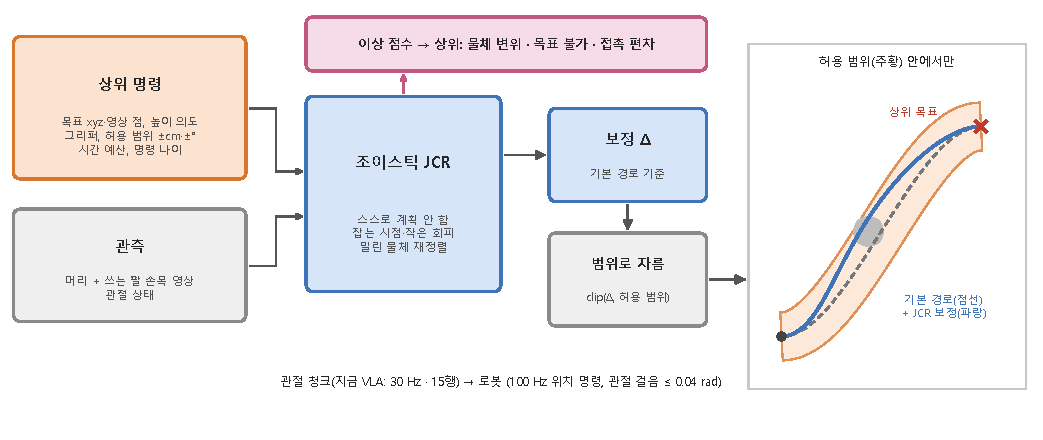
\includegraphics[width=\linewidth]{figures/f3_vla.pdf}
\caption{\textbf{조이스틱 JCR.} 코드 어댑터가 상위 출력에서 만든 명령(목적지 xyz, 대상 물체 마스크, 단계, 그리퍼 허용, 단계별 끌림 세기, 명령 나이)과 관측을 받아, 목적지로의 끌림 위에 보정을 TCP 변위 청크로 더하고 넓은 안전 범위만 자른다. 오른쪽: 끌림은 운반 중엔 약하고 잡기·놓기 근처에서 강하게 목적지로 당기며(파랑), 딱딱한 경로 관이 아니라 넓은 안전 범위(주황)만 지킨다. 이상 신호는 어댑터가 문장으로 바꿔 상위를 다시 부를 때 실어 보낸다.}
\label{fig:vla}
\end{figure*}

\paragraph{역할.} JCR(Joystick-Conditioned Reflex, 조이스틱 반사 정책)는 세 가지만 맡는다. (i) 조이스틱 따라가기, 곧 어댑터 명령 기준의 미세 조종, (ii) 잡기·놓기 시점, (iii) 접촉 여부 판단이다. 계획·단계 선택·목표 결정은 하지 않고 언어 명령도 받지 않는다(\cref{fig:vla}). 설계·데이터·학습·평가는 모두 상위가 명령을 주고 그 명령이 코드 어댑터를 거쳐 들어온다는 전제 위에 있다(\cref{sec:coupling}). 시뮬 참값 명령은 상한을 재는 데만 쓴다.

\paragraph{입력.} 머리·쓰는 팔 손목 영상과 고정된 짧은 문장(단계 문장 없음), 그리고 어댑터가 만든 명령 다섯 가지다. 목적지 xyz는 상위 점을 공용 코드가 깊이로 바꾼 값이다. 대상 물체 마스크는 명령 시점 머리 깊이에서 점 둘레 물체 영역의 3D 점을 구해 매 결정마다 머리·손목 영상에 다시 투영해 칠한 것이다(추적은 하지 않는다). 단계는 상위의 높이 의도를 그대로 옮긴 값(above·grasp·place·lift)이다. 그리퍼 허용은 상위 그리퍼 의도를 옮긴 이진값이다. 끌림 세기 $\kappa$는 단계별 규칙값(운반 중 0.3, 목표에서 먼 접근 0.5, 잡기·놓기 높이이거나 목적지 5\,cm 안이면 0.9)이다. 명령 나이는 명령이 나온 뒤 지난 시간이다. 고유 감각은 관절, 그리퍼 폭·전류(effort), 인과 후방 차분 속도, 현재 명령 관절이다. 단계 문장을 빼는 이유는 그리퍼 시점이 접촉이 아니라 문장에 붙기 때문이다(\cref{sec:evidence}).

\paragraph{출력과 권한.} 팔 행동은 현재 명령 TCP 기준의 변위 청크다(20\,Hz, 10행 = 0.5\,s, 0.2\,s마다 새 청크). 손끝 방향과 IK(중력 처짐 보정, 관절 한 걸음 0.04\,rad 이하)는 코드가 맡는다. 그리퍼는 행마다 \{유지, 닫기, 열기\} 사건을 내고, 접촉 확률 두 개(패드--대상, 예상 밖 접촉)를 낸다. 이상 신호는 별도 이진 머리(예상 밖 접촉, 대상 이동, 떨어짐, 명령 불일치, 복구 불가)와 멈춤 출력이며, 문턱은 보류 세트에서 등각(conformal) 방식으로 오탐률 5\,\%에 맞춘다~\cite{faildetect2025}. 실행되는 움직임은
\begin{equation}
  a_t = \mathrm{clip}\bigl(a^{\text{attr}}_t + \Delta_t,\ \mathcal{S}\bigr),
\end{equation}
이며 $a^{\text{attr}}$은 어댑터가 준 끌림 목표(아래), $\Delta_t$는 JCR 보정, $\mathcal{S}$는 딱딱한 경로 범위가 아니라 작업 공간 전체에 걸리는 넓은 안전 범위(10\,cm)다. 자름은 조종의 주된 수단이 아니라 마지막 안전 방어선이며, 허용 그리퍼 방향도 코드가 강제하므로 JCR가 틀려도 안전 범위 밖으로 벗어나지 않는다. 바탕 모델은 Qwen3-VL-4B~\cite{qwen3vl2025} LoRA 백본과 흐름 정합 행동 전문가이며, 전문가에서 백본으로 가는 기울기는 막는다~\cite{kinsulate2025}.

\paragraph{정답: 끌림 방향의 시뮬 참값.} 참값 물체 자세 $p^\ast$(특권 정보)와 목적지 $x^{\text{dest}}$의 차이를 $d = p^\ast - x^{\text{dest}}$로 두고, 보정 몫
\begin{equation}
  w = \frac{1}{1 + (|d| / \rho)^4}, \qquad \rho(\kappa) \in [\text{2\,cm at } \kappa{=}1,\ \text{7\,cm at } \kappa{=}0]
\end{equation}
로 정답 $c^\ast = x^{\text{dest}} + w\,d$를 만든다. 명령 점이 조금 틀렸으면($|d|$ 작음) $w \to 1$이라 끌림이 JCR를 실제 물체 쪽으로 거의 다 당기고(미세 조종), 명령 점이 전혀 다른 곳을 가리키면($|d|$ 큼) $w \to 0$이라 끌림은 명령 쪽에 머문다(따라가기). 한 정의로 두 역할이 나오고, 권한은 늘 상위에 있다. $w < 0.5$이면 명령 불일치 신호를 올린다. 안전 범위 $\mathcal{S}$(10\,cm)만 코드가 자른다. 참값 청크는 최소 저크 모양(속도 $\le$ 0.08\,m/s, 가속 $\le$ 0.32\,m/s$^2$)이고, 닫기 참값은 특권 쥐기 술어가 처음 참이 되는 틱, 열기 참값은 놓기 자세 1\,cm 안, 접촉 참값은 시뮬 접촉 센서 힘 $>$ 0.1\,N이다. 스냅샷마다 가짜 명령 넷(명령 점 오차 먼 구간 0.5--8\,cm, 근접 0.3--2\,cm)에 참값 청크를 짝지은 반사실 분기를 넣고, 분기는 시뮬 재생으로 실행 가능성을 확인한다(계획 대 실측 TCP 변위 차 중앙 $\le$ 3\,mm).

\paragraph{조종 방식 비교(JCR1-0A/B/C).} 위 $w$ 규칙(B, 끌림만)과 함께 두 비교 팔을 같은 데이터에 함께 싣는다: A 딱딱한 범위(정답은 목적지 3\,cm 공에 투영, 실행은 목적지 3\,cm + 경로 관 4\,cm로 자름), C 섞기(B의 점을 다시 3\,cm 공에 투영해 정답으로, 실행은 3\,cm로 자름). 편마다 실행 규칙을 A/B/C 중 무작위로 골라 세 규칙의 상태 분포를 함께 덮되, 표본마다 세 규칙의 정답을 모두 저장해 같은 데이터로 세 모델을 학습한다(\cref{sec:eval}).

\paragraph{자기 롤아웃 재라벨.} 참값은 상태만의 함수이므로 JCR 자신이 돈 롤아웃의 방문 상태에서 다시 계산해 붙인다. 라벨을 내는 쪽은 학습된 정책이 아니라 특권 상태 함수이므로 교사 정책이 아니다. 라운드마다 기초 데이터와 모든 재라벨 데이터를 합쳐 처음부터 다시 학습하며, 교정 데이터만으로 이어 학습하지 않는다. 이 반복이 폐루프에서 생기는 상태 분포 이동을 없애는 수단이다.

\paragraph{실패와 외란.} 실패·외란은 버리지 않고 일부러 만든다. 물체 밀기, 미끄러짐, 장애물, 잡기 직전 대상 흔들기, 그리고 어댑터를 거친 상위 명령의 점 오차·의도 오류·지연·도중 교체다. 규칙은 문헌을 따른다.
\begin{itemize}
  \item 실패 편에서 실행된 행동은 행동 복제 라벨로 쓰지 않는다. 방문 상태만 남기고 행동은 시뮬 참값 교정으로 바꾼다~\cite{crdagger2025,rac2025}. 이득 토큰 조건화~\cite{recap2025}는 쓰지 않는다.
  \item 정상 흐름은 절반 이상으로 두고, 교란 구간 안에서는 `범위로 복귀' 대 `과제 진행'을 1:1--1:2로 맞춘다. 교란 뒤 3\,s 안에 복구하지 못한 긴 꼬리는 자른다~\cite{rac2025}.
  \item 교란 크기는 JCR 자신의 오차 분포와 성공률에 맞춰 단계적으로 키운다~\cite{laskey2017dart}.
  \item 복구 불가 상태(탁자 밖으로 떨어짐, 넘어져 닿을 수 없음, 관절 한계)는 참값 교정기로 이어 돌린 반사실 롤아웃으로 판정하고, 정답은 억지 보정이 아니라 `이상 신호 + 멈춤'이다. 다시 계획하는 것은 상위다.
  \item 관측으로 알아볼 수 없는 교정(숨은 미끄러짐 등)은 행동 정답 대신 이상 신호로 보낸다.
\end{itemize}
틱마다 단계, 명령원, 외란 종류·시점, 편 결과를 남겨 같은 기록을 상위의 진행 평가·실패 감지 학습에도 쓸 수 있게 한다.

\paragraph{명령원.} 편의 30\,\%는 시뮬 참값 명령, 70\,\%는 상위 흉내 명령으로 만들고, 둘 다 코드 어댑터를 거쳐 JCR에 들어간다(\cref{sec:coupling}). 상위 흉내 명령은 본 35B 오프라인 평가에서 잰 경험 분포(점 오차, 동작 오류율, 호출 지연)를 머리 영상 픽셀 $\rightarrow$ 깊이 $\rightarrow$ xyz 경로로 주입하고, 갱신 간격 2--6\,s(상위가 생각하는 1--3\,s 구간의 늘어난 명령 나이 포함), 도중 교체 10\,\%를 더한다.

\paragraph{학습 4단계.} 정답은 모두 시뮬 참값(특권 정보로 계산)이다. 상위는 동결해 재학습하지 않으므로 네 단계 모두 JCR만 갱신한다.
\begin{enumerate}
  \item \textbf{단독:} 참값·상위 흉내 명령 위에서 교란 장면의 참값 보정을 배우고, 자기 롤아웃 재라벨을 되풀이한다. 데이터 관문은 보정이 안전 범위 안인지, 관절 걸음 $\le$ 0.04\,rad인지, 분기 실행 검증, 접촉 라벨 프레임 검수다.
  \item \textbf{상위 오차 흉내:} 주입 비중과 크기를 본 35B 최적 체크포인트의 오차·지연 분포로 맞춘다.
  \item \textbf{실제 상위와:} 동결한 실제 상위 + 어댑터를 붙여 돈 기록에서 참값 보정으로 다시 학습해, 연결 지점의 분포 차이를 없앤다.
  \item \textbf{반복 정착:} 라운드마다 실제 상위+어댑터 기록을 다시 모아 JCR만 계속 갱신하고, 매 바퀴 같은 시드 2$\times$2로 연결 손실을 잰다. 더 줄지 않으면 멈춘다(\cref{sec:mesh}).
\end{enumerate}
단독 성능표(참값 명령·상위 흉내 명령에서의 성공률, 교란 복구율, 접촉·이상 신호 정밀도·재현율, 그리퍼 시점 오차)는 1단계 뒤에 만들고, H-J 비교의 기준선이 된다(\cref{sec:eval}).
